
%(BEGIN_QUESTION)
% Copyright 2011, Tony R. Kuphaldt, released under the Creative Commons Attribution License (v 1.0)
% This means you may do almost anything with this work of mine, so long as you give me proper credit

A technique to measure {\it average} temperature using multiple sensors involves paralleling multiple thermocouples, using ``swamping resistors'' to join them to a single transmitter:

$$\includegraphics[width=15.5cm]{i02354x01.eps}$$

First, explain what the purpose of these swamping resistors is -- why not just simply parallel the three thermocouples directly?  Second, determine what will happen if one of these swamping resistors were to fail open.

\vskip 20pt \vbox{\hrule \hbox{\strut \vrule{} {\bf Suggestions for Socratic discussion} \vrule} \hrule}

\begin{itemize}
\item{} Describe a practical application where we might need to have an {\it average} temperature measurement of three different locations than a single-point measurement.
\item{} Where should thermocouple wire be used in this circuit, and where is it appropriate to use copper wire?
\item{} Will the presence of these swamping resistors impact the reference junction compensation?  Why or why not?
\end{itemize}

\underbar{file i02354}
%(END_QUESTION)





%(BEGIN_ANSWER)

A circuit to jog your memory on this concept is the {\it noninverting summer}, designed to sum (add) three analog voltage signals:

$$\includegraphics[width=15.5cm]{i02354x02.eps}$$

At the noninverting input of the opamp is a set of three resistors functioning as a {\it passive averager}, to input the average of the three sources' voltage values to the opamp's noninverting input.  It is this ``averaging'' resistor network which has relevance to the thermocouple circuit shown in the question.  Swamping resistors are necessary to ``even out'' the otherwise disparate thermocouple wire resistances, so that the voltage signal received is a more fairly-weighted average that it would be otherwise.

\vskip 10pt

If a swamping resistor happens to fail open, that thermocouple no longer has any effect on the average.  In other words, the output voltage signal becomes the average of the remaining two thermocouples.

%(END_ANSWER)





%(BEGIN_NOTES)





\vskip 20pt \vbox{\hrule \hbox{\strut \vrule{} {\bf Virtual Troubleshooting} \vrule} \hrule}

This question is a good candidate for a ``Virtual Troubleshooting'' exercise.  Presenting the diagram to students, you first imagine in your own mind a particular fault in the system.  Then, you present one or more symptoms of that fault (something noticeable by an operator or other user of the system).  Students then propose various diagnostic tests to perform on this system to identify the nature and location of the fault, as though they were technicians trying to troubleshoot the problem.  Your job is to tell them what the result(s) would be for each of the proposed diagnostic tests, documenting those results where all the students can see.

During and after the exercise, it is good to ask students follow-up questions such as:

\begin{itemize}
\item{} What does the result of the last diagnostic test tell you about the fault?
\item{} Suppose the results of the last diagnostic test were different.  What then would that result tell you about the fault?
\item{} Is the last diagnostic test the best one we could do?
\item{} What would be the ideal order of tests, to diagnose the problem in as few steps as possible?
\end{itemize}


%INDEX% Measurement, temperature: parallel thermocouples
%INDEX% Measurement, temperature: thermocouple

%(END_NOTES)

